 
\section{Preliminary Results}
\label{sec:results}

\begin{itemize}
\item need a coherent story here (organize as a story!)
\item show some optimization examples, provide story
\item character of solution(s), observations
\item define how we measure flux!
\end{itemize}



The computer simulations of this proposal are intended to discover the
optimal system configuration for a range of scenarios and system
sizes. The results of these simulations will be used as input for the
design of a pilot site in Mesa, Arizona, and eventually, over a range of
scenarios and system sizes. 

  \begin{figure}[!htb]
   \begin{center}
    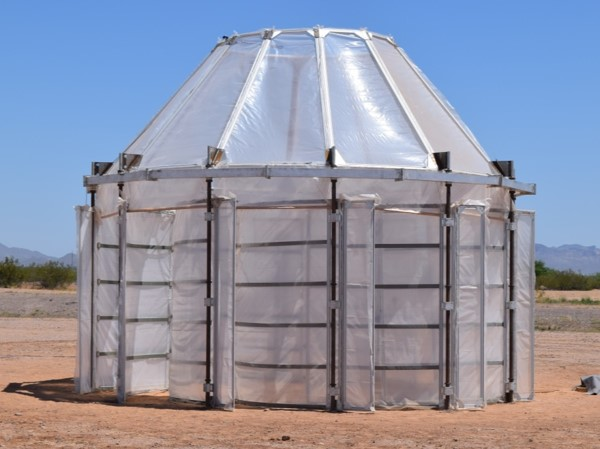
\includegraphics[width = 12 cm]{figs/sov_field}
    \caption{A photo of the field configuration, during the June 2015
    Field Test.}
    \label{fig:field_real}
   \end{center}
  \end{figure}

Potential Temperature is defined as,\todo{where are you using this fellow}
\begin{equation}
  \theta(x,y,z) = T(x,y,z) -T_{in}(z) 
\end{equation}

\subsection{Thermal Only}

While ambient winds in the field do impact system performance, it is
also illuminating to consider an idealized scenario with natural convection
driven only by thermal instabilities. Investigating this baseline,
thermal-only flow is intended to optimize the SoV apparatus to form a
strong thermal plume even in the absence of wind. After a system is
engineered to form a strong thermal plume, we can investigate to ensure
that the existing thermal vortex will be strengthened by the addition of
winds.

Two hundred Watts?\todo{fix these shitty figures}

  \begin{figure}[htp]

   \centering   
   \begin{minipage}{0.47\textwidth}
    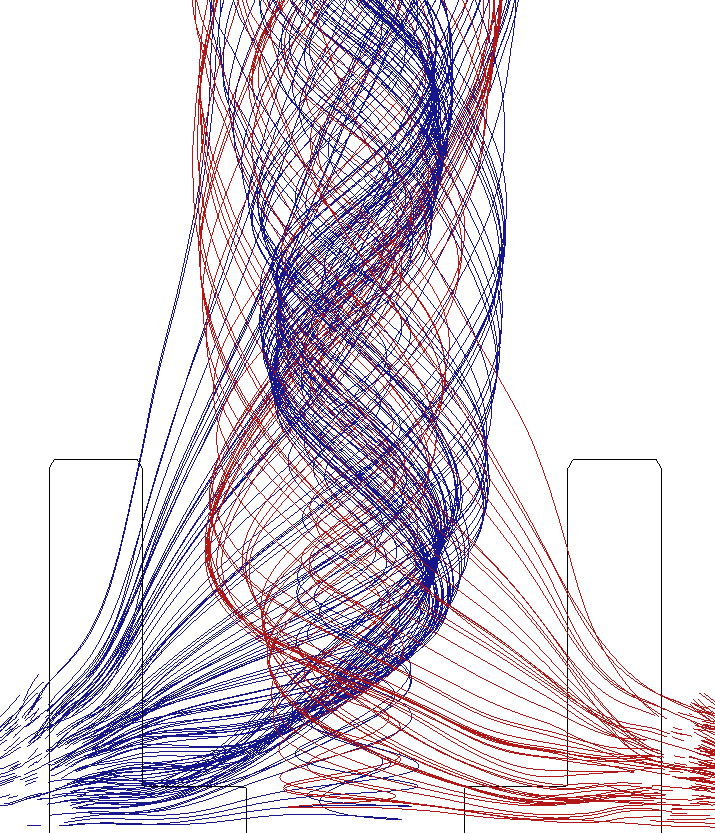
\includegraphics[width =0.9\textwidth]{figs/entrainment}%
    \caption{This is an image of particles seeded and advanced
    through a velocity field. One can observe a tight inner vortex with
    significant azimuthal velocity formed through the bottom tier of
    vanes, as well as a broader region of entrained fluid through the
    second tier.} 
   \end{minipage}   
   
   \centering
   \begin{minipage}{0.47\textwidth}
    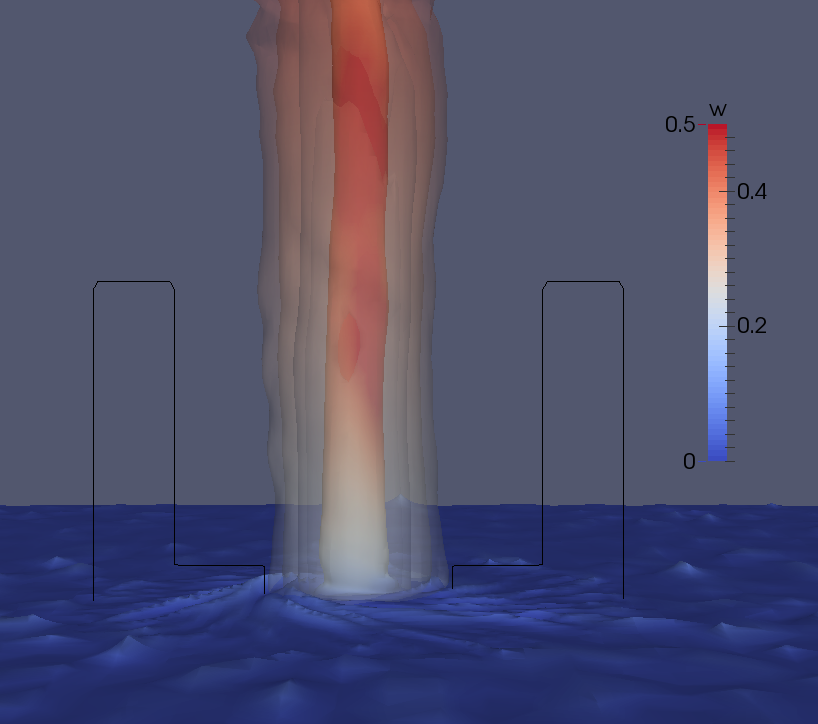
\includegraphics[width =0.9\textwidth]{figs/3d}
    \caption{This image depicts isocountours of the inner thermal core
    visible through semi-transparent contour around azimuthal velocity,
    colored by vertical velocity. }
   \end{minipage}      
   \label{fig:entrain}  
  \end{figure}



Rotating air induces low pressure core, as observed in:
Dust Devils

%
% conclusion of thermal only
%
While these results are promising, the thermal plume is relatively
narrow compared to the diameter of the device. It is desirable to
broaden the thermal plume, as this in turn creates a larger vertical
momentum flux due to the effects of buoyancy. This will presumably
entrain more surrounding fluid, driving it through the vanes and
imparting kinetic energy to the flow. The kinetic energy grows as the
square of the radius, so any broadening of the vortex core can greatly
enhance the kinetic energy flux. However, the general physical
mechanisms that determine the thermal plume's thickness are not
presently understood. 

\subsection{Wind}

Discussion thermal + wind

\subsection{Optimization}

%
%\subsection{Character of the Solution}
%
%Talk about how the vortex transitions from phase 1 to 2, etc. 
